Understanding the time profile of a beam spill is crucial for various reasons in accelerator physics and radiation testing of electronic devices. One key aspect is the flux, which refers to the number of particles per square centimeter per second (p/cm²·s) that pass through a device over a given period of time. A high flux of particles during a spill can lead to a high number of Single Event Effects (SEE) in electronic devices under test, which can degrade and fail sooner than if they were exposed to a lower flux over the same period of time. In radiation testing, a constant flux is preferred to simplify the analysis, however, a non-uniform spill with an accurate time profile and flux measurement as a function of time is also useful. This chapter will present a detailed analysis of the time profile of the slow extracted spills that occurred during the November 2022 run. The analysis will include a description of the instruments and methods used to gather data, a presentation of the results, and a discussion of the implications of these results for future beams.

\subsubsection{Instruments and location}

Seven instruments are used to measure the time profile. These are the gas scintilator, the Secondary Emission Chambers (XSECs) (23/70/94), the Ionization Chamber XION(71/94) and the diode. The numbers refer to the position of the instrument in the transfer line in a sequential order. The instruments in position 94 are the closest to the device under test.

The Beam Current Measurement based on Gas (BCGAA), previously known as a longitudinal spill detector (LSD), utilizes nitrogen gas to detect beam-induced ionization photons. The collected photons generate an electric signal, which is then amplified and sampled using a photo-multiplier (PM) to accurately measure the beam current.

The XSECs are used to measure the number of particles passing through the accelerator. They work by directing the beam through a series of thin metal foils, such as aluminum. When the beam interacts with the foils, it generates secondary electrons which are then detected by a charge-integrating circuit. The integrated current is proportional to the number of particles passing through the foils and is often converted into counts for ease of data transmission. XSECs have varying sensitivities depending on their design and number of foils. For instance, in the T08 beamline, T08.XSEC070 (which has 10 foils) has a sensitivity four times higher than T08.XSEC094 (which only has 2 foils) \cite{ravotti_calibration_2022}.

An example of the spill time profile of the XSEC70 is shown in Fig. \ref{fig:spill_time_profile1}.

\begin{figure}[!htb]
\centering
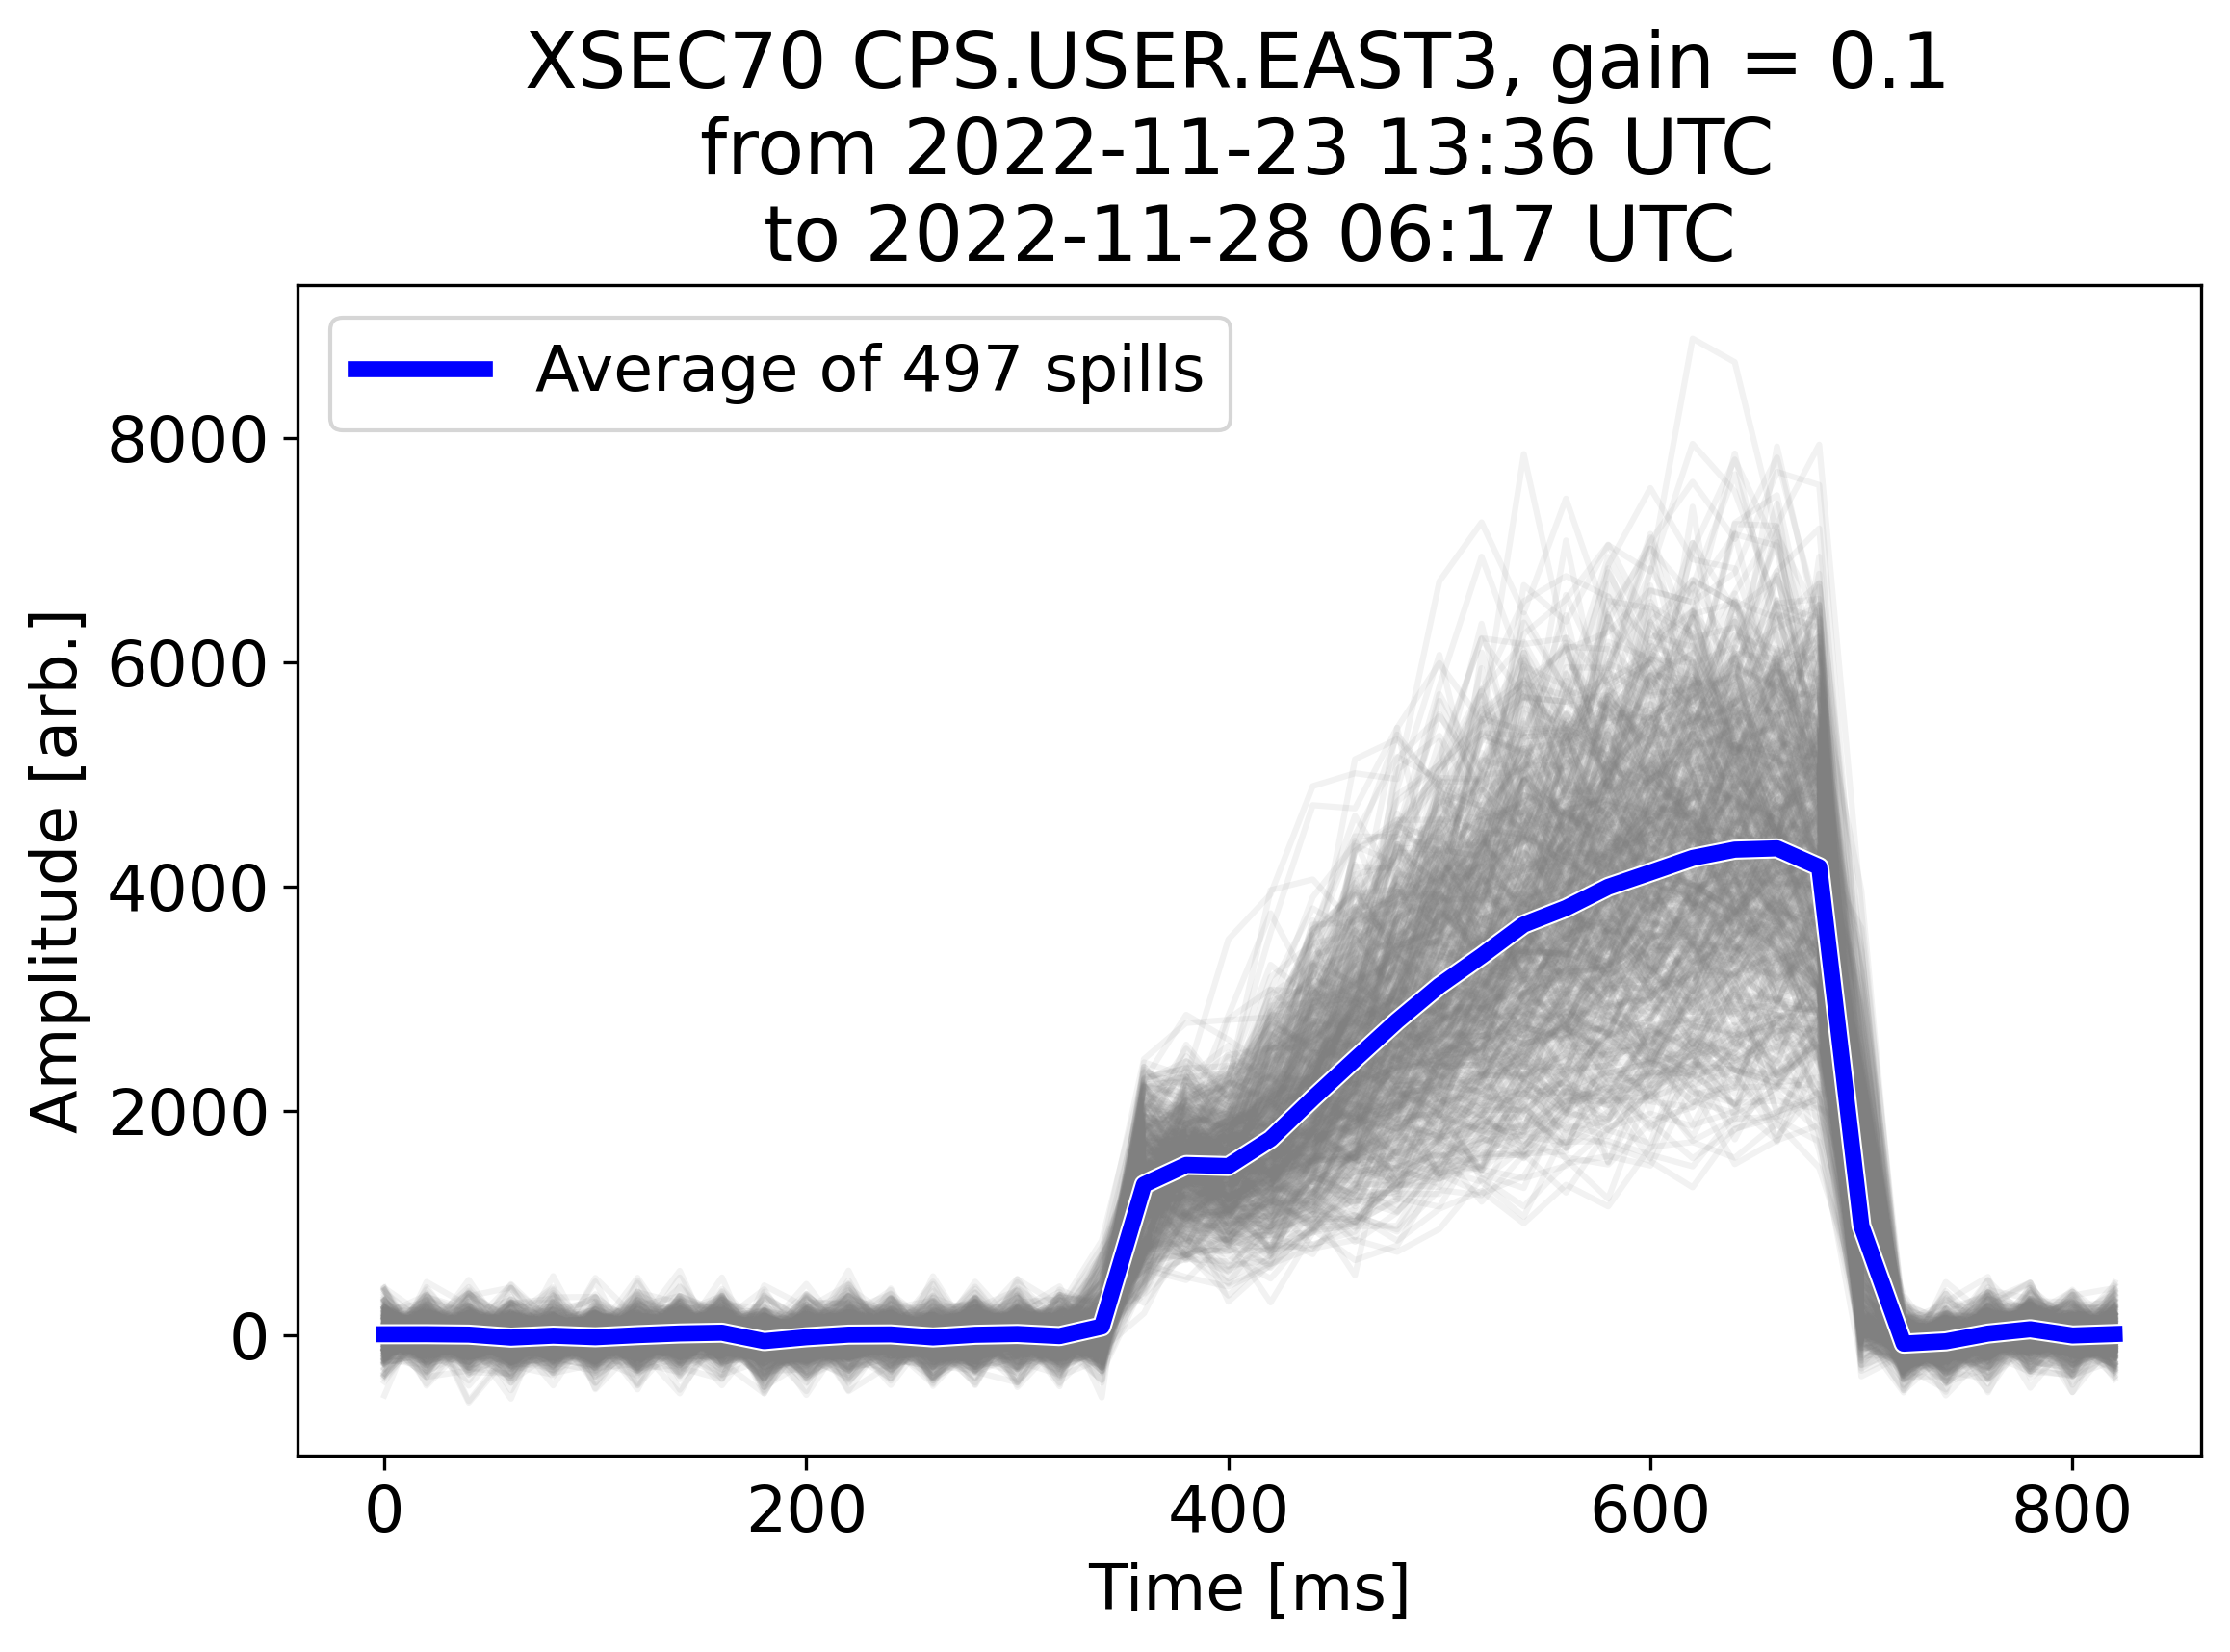
\includegraphics[width=0.6\textwidth]{images/spill_profile_xsec_CPS.USER.EAST3_0.1_1.png}
\caption{Single spills are plotted in gray and the average of the spills in plotted in blue.}
\label{fig:spill_time_profile1}
\end{figure}

\begin{figure}[!htb]
\centering
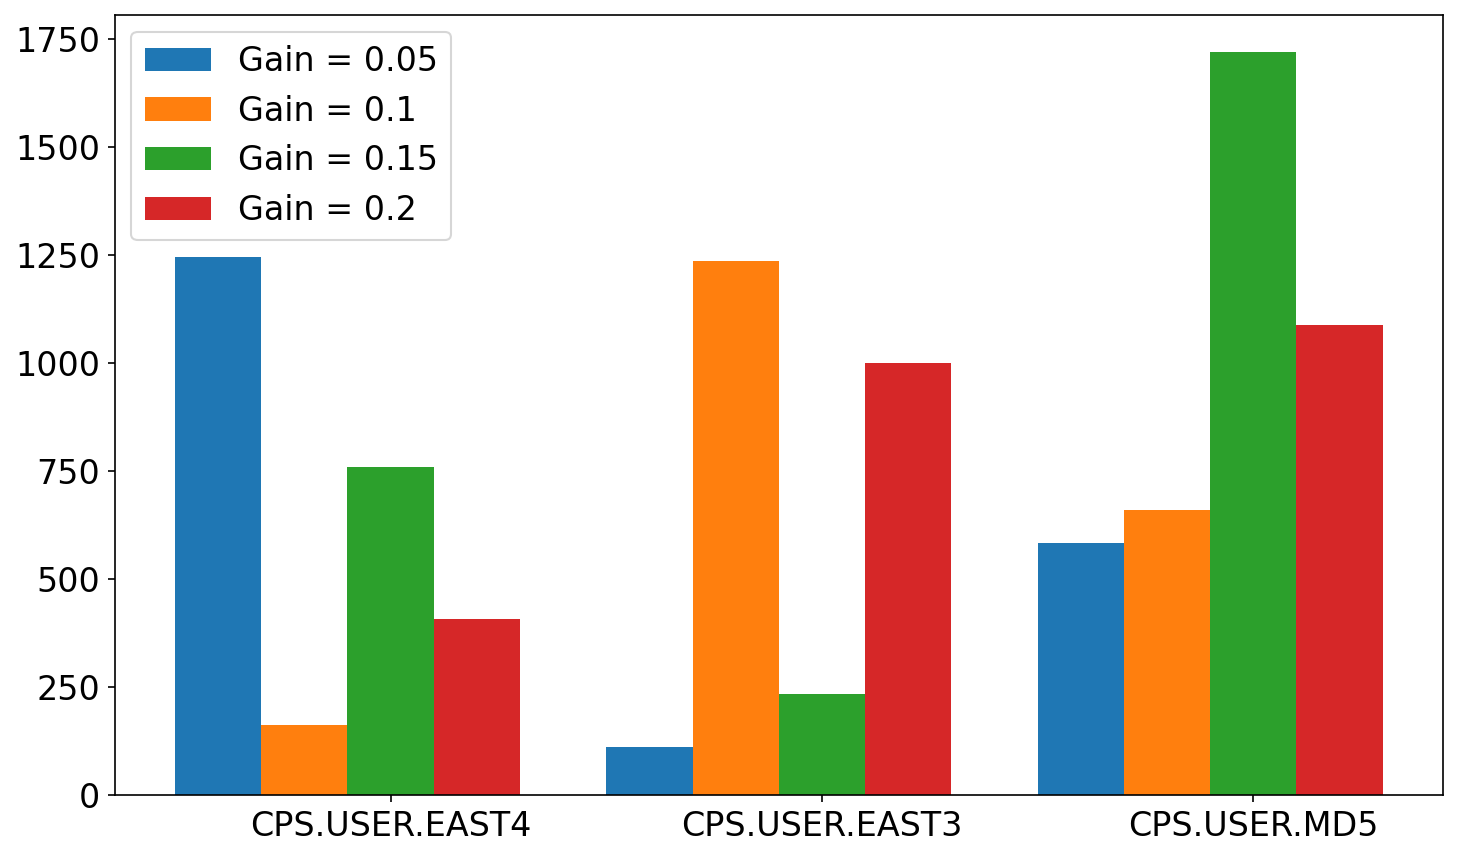
\includegraphics[width=0.6\textwidth]{images/bar_chart_gain_energy.png}
\caption{Spill time profile}
\label{fig:spill_time_profile2}
\end{figure}

\begin{figure}[!htb]
\centering
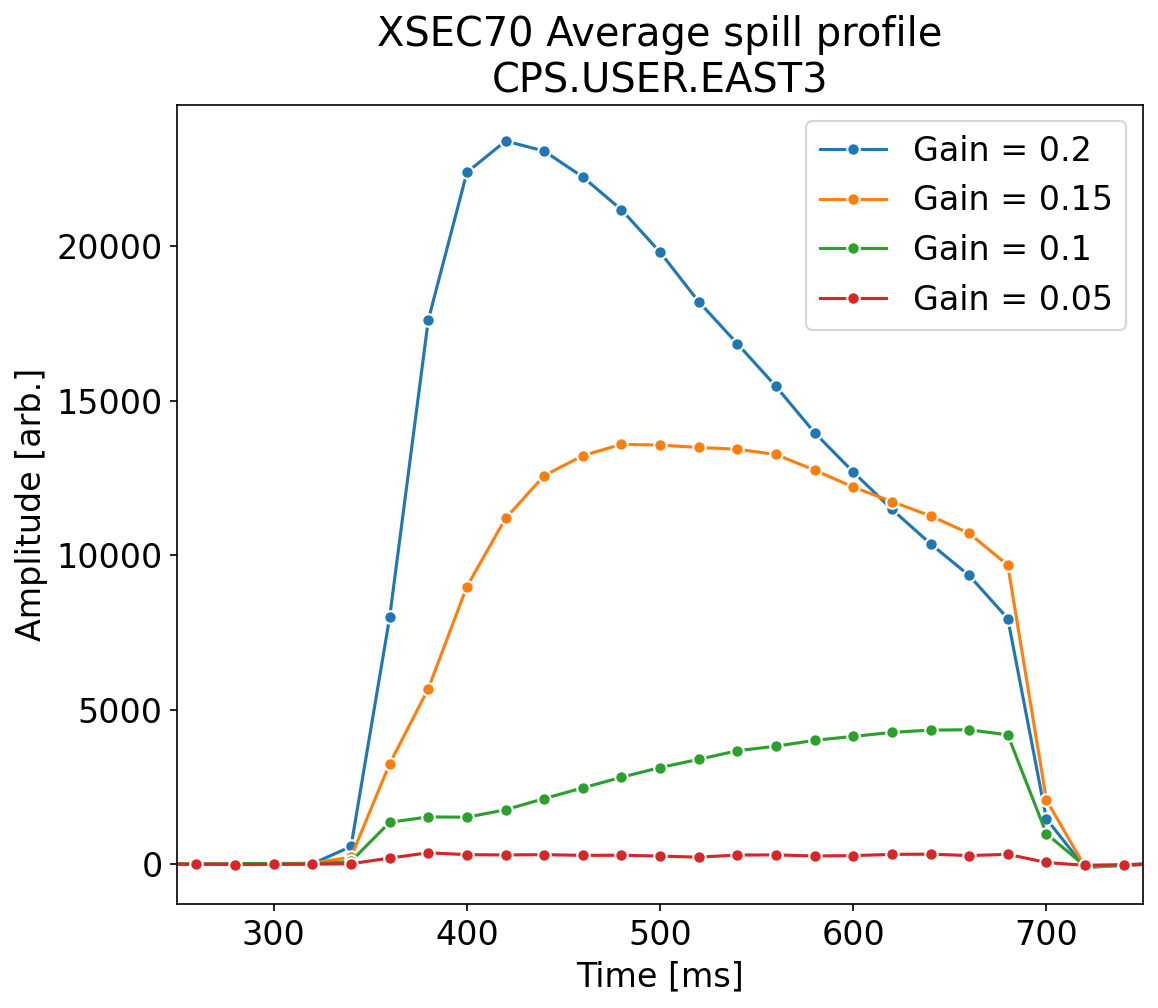
\includegraphics[width=0.6\textwidth]{images/spill_profile_xsec70_average_EAST3.png}
\caption{Spill time profile}
\label{fig:spill_time_profile3}
\end{figure}

\begin{figure}[!htb]
\centering
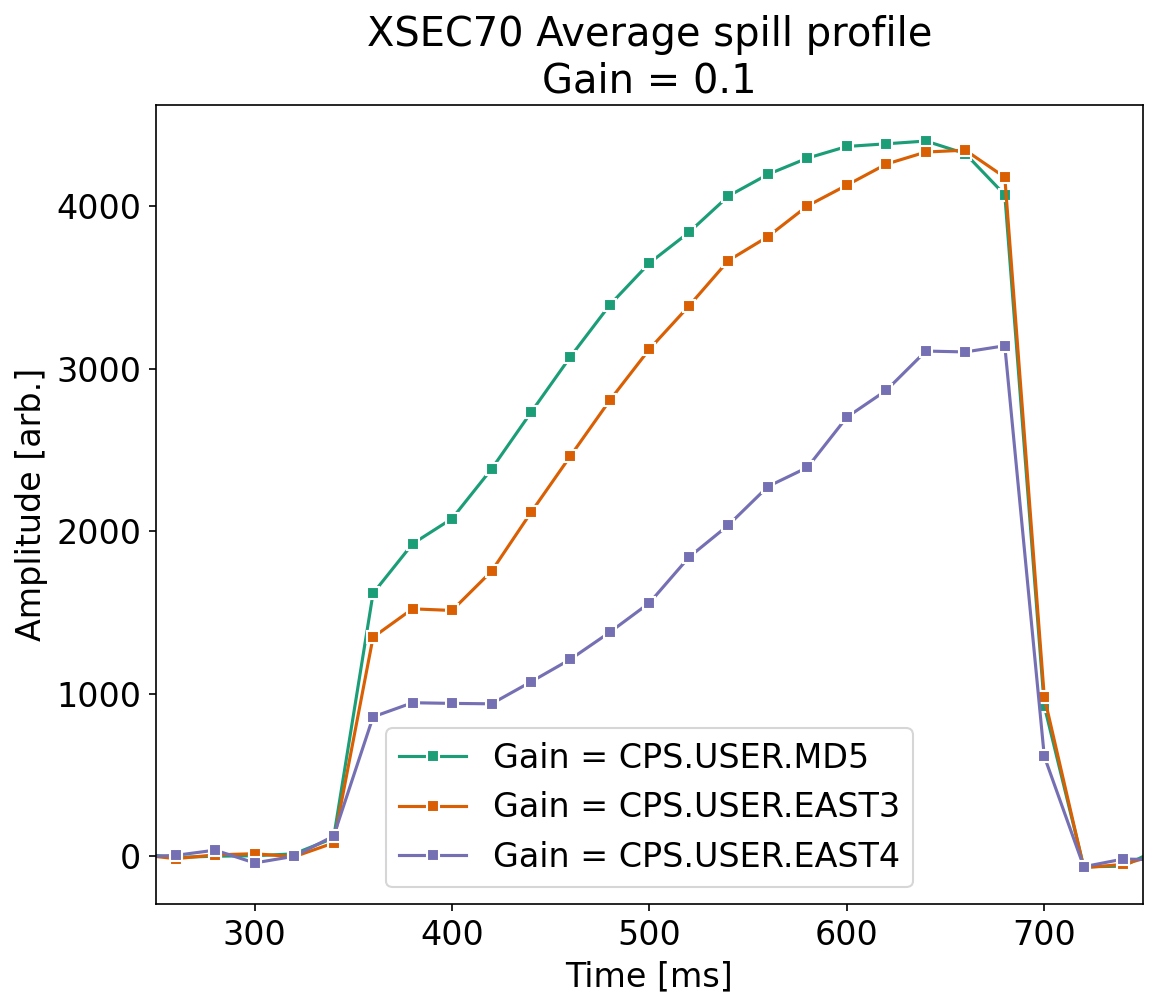
\includegraphics[width=0.6\textwidth]{images/spill_profile_xsec70_average_gain_0.1.png}
\caption{Spill time profile}
\label{fig:spill_time_profile4}
\end{figure}

\subsubsection{Beam Time Structure}
\label{beam_time_structure}

The beam under study displays a complex frequency structure, with slow and fast frequencies present. To deliver a slow extracted beam, the Radio Frequency Knock Out (RFKO) technique is employed. This involves generating a chirp waveform with a predetermined repetition rate. However, in 2022, the Qmeter2 software that controls the voltage on the RF plates limited the maximum chirp repetition rate to 1 millisecond intervals, see Fig. \ref{fig:RFKO_chirp_explanation}. As a result, a spectral line at 1 kHz is produced. Additionally, a fast spill structure is observed at the fractional tune of the third integer, corresponding to frev/3. The revolution frequencies for the 650, 750, and 1000 MeV beams are 385, 397, and 417 kHz, respectively, resulting in spectral lines at approximately 130 kHz and their associated harmonics. The gas scintillator used for detection has a Nyquist frequency of 1 kHz due to its 0.5 ms sampling rate, capturing only the lowest frequency lines. Conversely, the diode's much faster sampling rate of 0.5 $\mu$s enables it to detect both slow and fast frequencies, as seen in Fig. \ref{fig:spill_fft_diode}. Future runs could benefit from adjusting the sampling granularity to be coarser or finer, down to the nanosecond scale.

\begin{figure}[!htb]
\centering
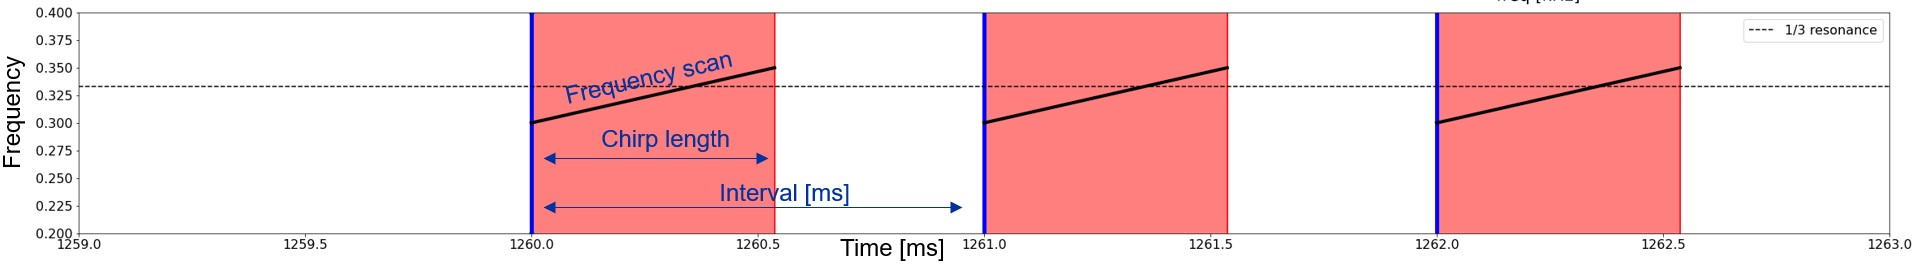
\includegraphics[width=1.0\textwidth]{images/SPILL_TIME_PROFILE/RFKO_chirp_explanation.jpg}
\caption{The RF chirps at a repetition rate of 1 kHz during a chirp length. Although a chirp length that is not a power of 2 would be more optimal for our needs, we are currently forced to use a power of 2 by design of the Qmeter2 software that controls the voltage on the RF plates. As shown in the diagram, the RF frequency ramps up during the chirp and repeats the ramping at every chirp, producing a quasi sawtooth signal. This signal blows up the emittance and extracts the beam.}
\label{fig:RFKO_chirp_explanation}
\end{figure}

\begin{figure}[!htb]
\centering
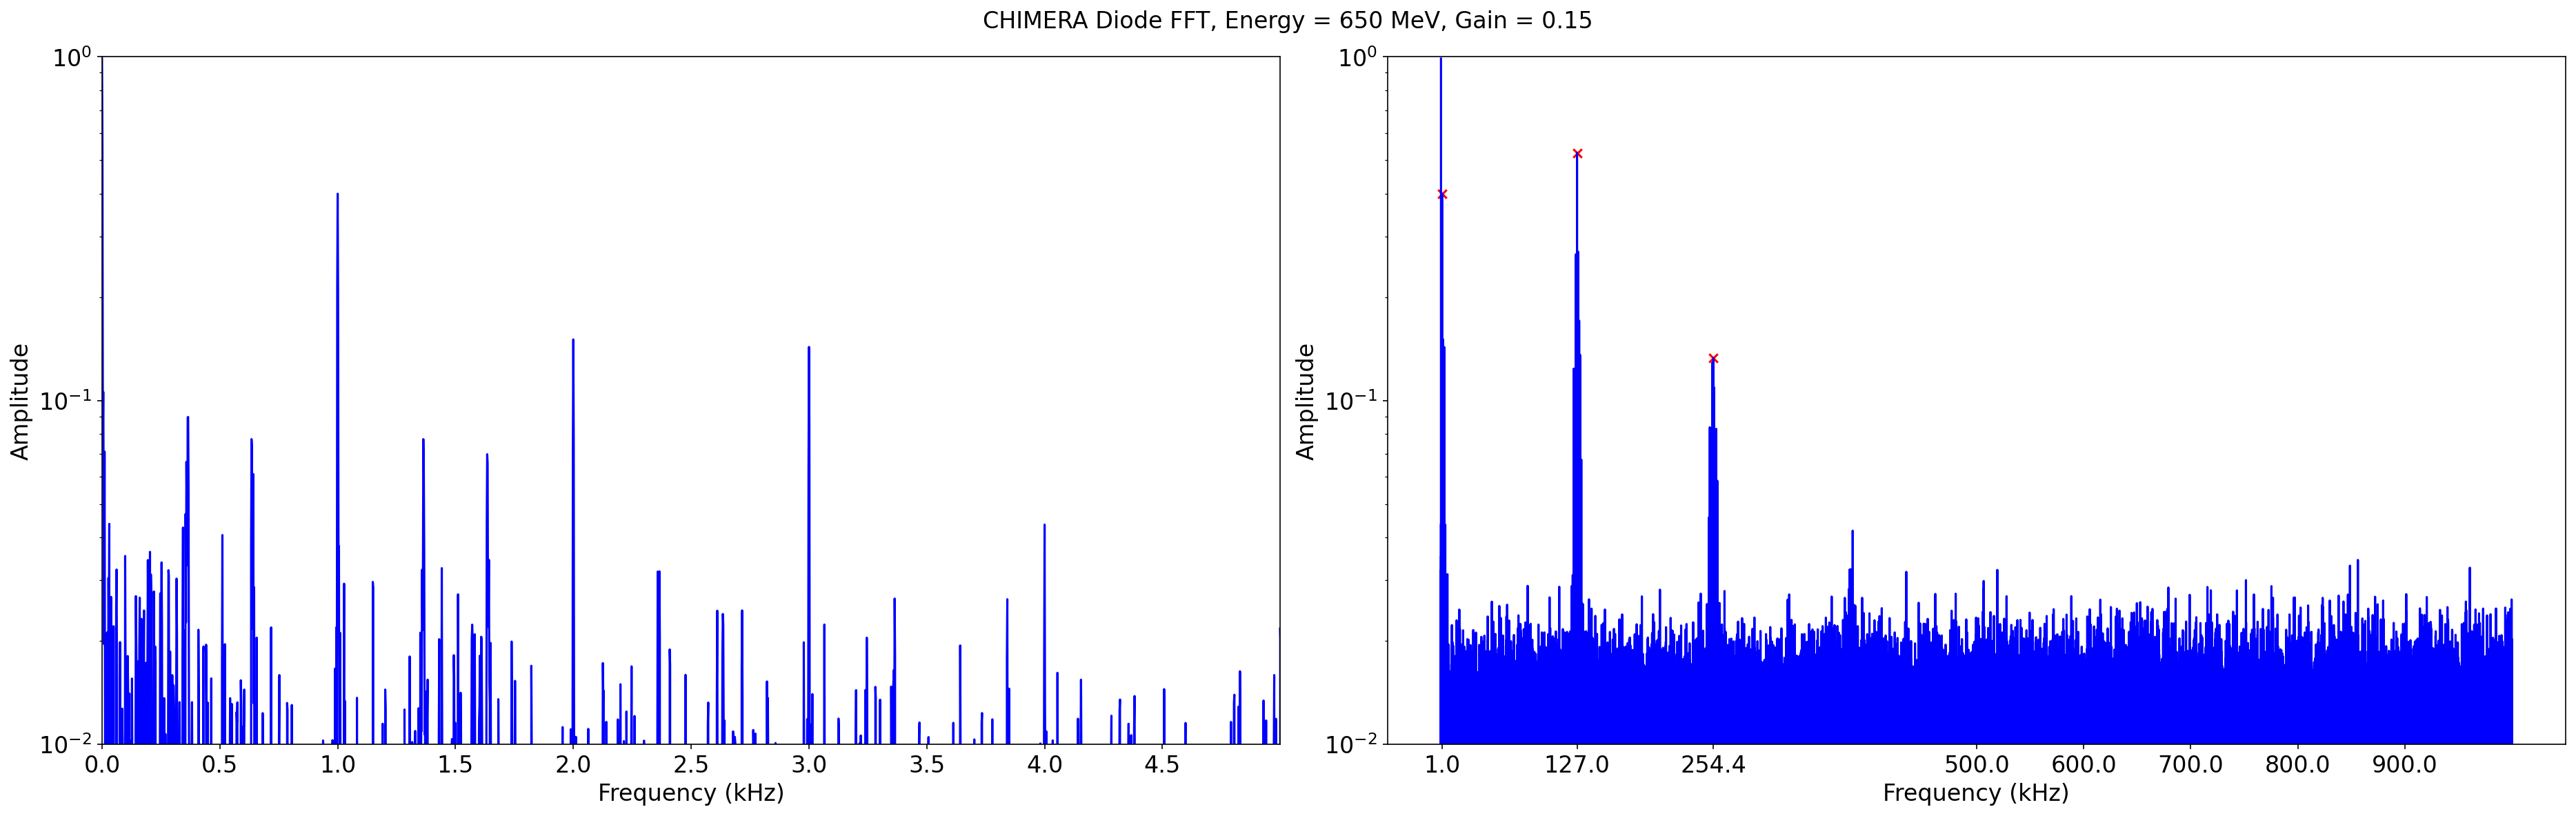
\includegraphics[width=0.9\textwidth]{images/SPILL_TIME_PROFILE/CHIMERA_diode_FFT_two_scales.png}
\caption{FFT of a 650 MeV spill at 0.15 gain measured with the diode in CHARM. The left plot shows the harmonics of the 1 kHz RFKO chirping technique, while the right plot displays the 130 kHz signal and its harmonics.}
\label{fig:spill_fft_diode}
\end{figure}

The fast frequencies are correlated with the revolution frequency of the beam (FREV), which varies with the beam energy, as listed in Table \ref{table:frev}.

\begin{table}[]
\centering
\begin{tabular}{lll}
USER           & frev [kHz] & frev/3 [kHz] \\
\hline
CPS.USER.EAST4 & 417.7      & 139.2        \\
CPS.USER.EAST3 & 397.8      & 132.6        \\
CPS.USER.MD5   & 385.4      & 128.5       
\label{table:frev}
\end{tabular}
\end{table}

During our testing phase, we employed a signal generator to send custom signals to the TFB plates, which could be remotely controlled using Python scripts. However, we did not use it during the November run. To mitigate the impact of low frequencies, we experimented with chirping at a higher repetition rate and pulsing in a continuous sawtooth signal, which effectively damped and broadened the chirp excitation signal. In order to address the higher frequencies induced by the revolution frequency, one idea we are considering is to inject more bunches around the machine and attempt to debunch the beam for longer durations.